\documentclass[a4paper]{article}

% Required package
\usepackage{tikz}
\usetikzlibrary{mindmap} % Mindmap drawing library  %used by mindmap.tex

\usepackage[
backend=biber,
style=alphabetic,
]{biblatex}
\addbibresource{refs.bib} %Imports bibliography file
\usepackage[utf8]{inputenc}
\usepackage{graphicx}
\usepackage{float}
\graphicspath{ {./images/} }
\usepackage{multicol}
\usepackage{setspace}

%% Language and font encodings
\usepackage[english]{babel}

\usepackage{booktabs}
\usepackage{tabu}
\usepackage[T1]{fontenc}

%% Sets page size and margins
\usepackage[a4paper,top=3cm,bottom=2cm,left=3cm,right=3cm,marginparwidth=1.75cm]{geometry}

%% Useful packages
\usepackage{amsmath}
\usepackage{graphicx}
%\usepackage{apacite}
\usepackage[colorinlistoftodos]{todonotes}
\usepackage[colorlinks=true, allcolors=blue]{hyperref}

\title{A Survey on Advanced Machine Learning (ML) techniques to Protect Smart Grid Against Cybersecurity Breaches }
\author{Raymond \textbf {Rono} Cheruiyot \\ Department of Computer Science}
\date{13 September 2022}

\begin{document}
\maketitle
\tableofcontents
\section{Mind Map}

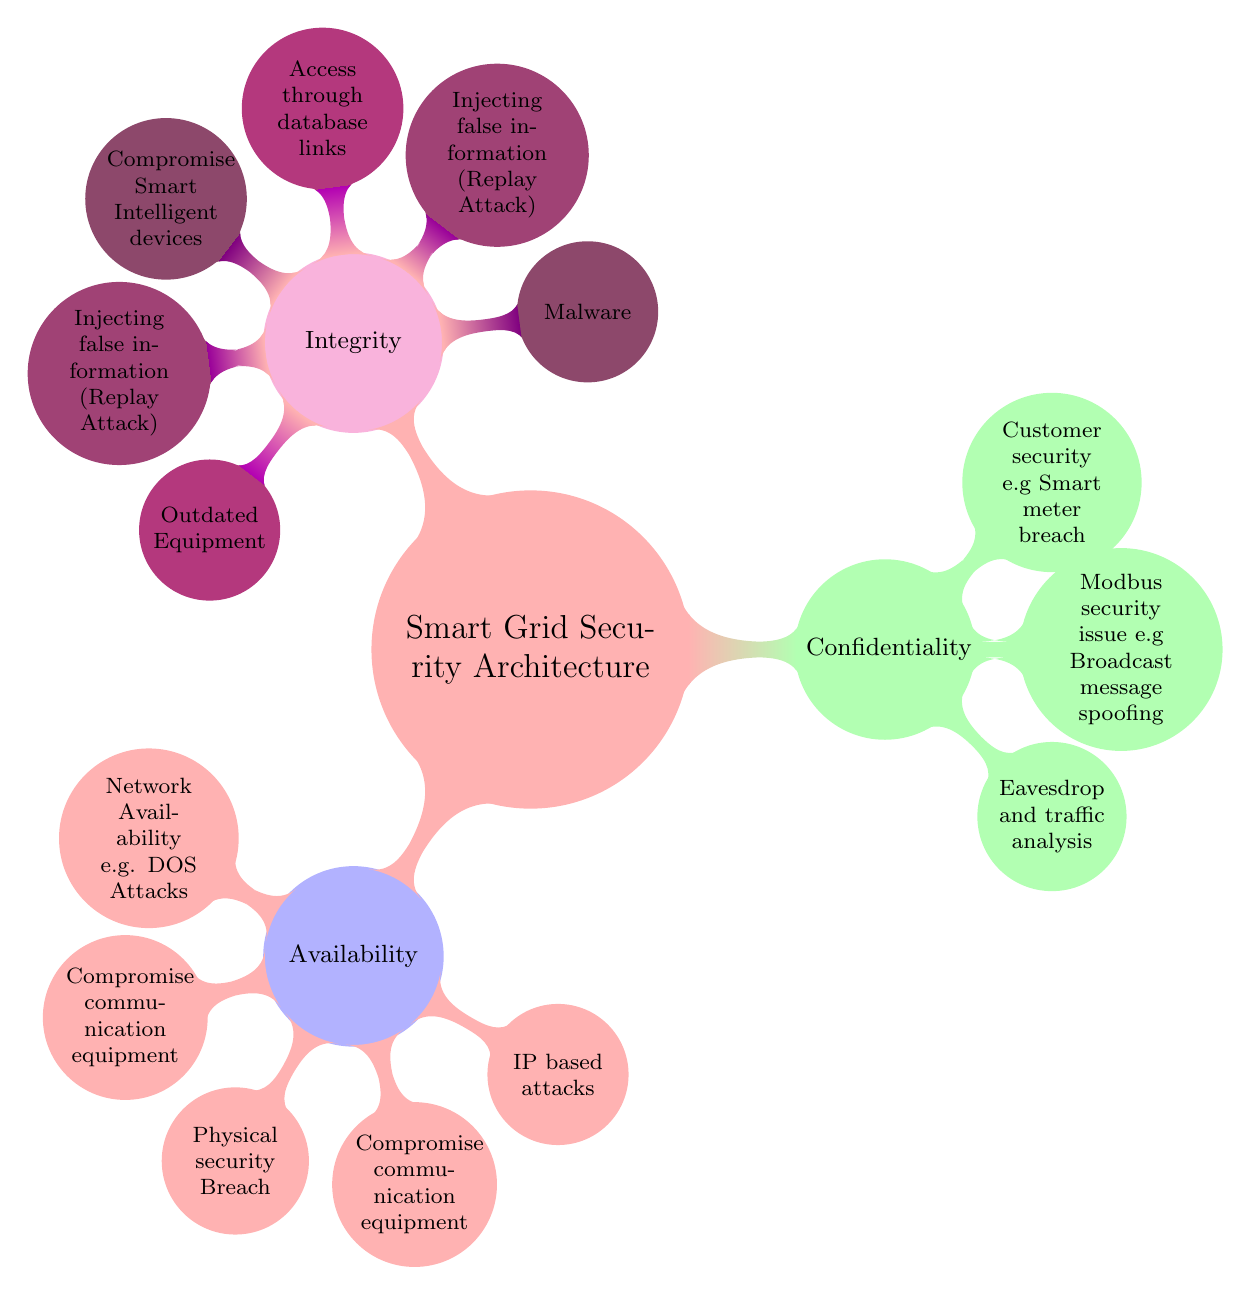
\begin{tikzpicture}[
    mindmap,
    concept color = red!30, 
    every node/.style = {concept}, 
    grow cyclic,
    level 1/.append style = {
        level distance = 4.5cm,
        sibling angle = 120
    },
    level 2/.append style = {
        level distance = 3cm,
        sibling angle = 45}
]

\node {Smart Grid Security Architecture}
        child {node [concept color = blue!30] {Availability}
            child {node {Network Availability e.g. DOS Attacks}}
            child {node {Compromise communication equipment}}
            child {node {Physical security Breach}}
            child {node {Compromise communication equipment}}
            child {node {IP based attacks}}
        }
        child [concept color = green!30] {node {Confidentiality}
            child {node {Eavesdrop and traffic analysis}}
            child {node {Modbus security issue e.g Broadcast message spoofing}}
            child {node {Customer security e.g Smart meter breach}}
        }
        child {node [concept color = magenta!30] {Integrity}
                child [concept color = magenta!50!black] {node {Malware}}
                child [concept color = magenta!60!black] {node {Injecting false information (Replay Attack)}}
                child [concept color = magenta!70!black] {node {Access through database links}}
                child [concept color = magenta!50!black] {node {Compromise Smart Intelligent devices}}
                child [concept color = magenta!60!black] {node {Injecting false information (Replay Attack)}}
                child [concept color = magenta!70!black] {node {Outdated Equipment}}
        };

     %\child {Cybersecurity Threats Against the Smart Grid}
\end{tikzpicture}


\section{Question: Describe your learning/process so far on the survey paper.}

\begin{itemize}
    \item Step 1: Selecting the representative papers 
    \\The first step is to select the most relevant representative papers that are within the scope of “Machine Learning” + “Security” + “Smart Grid.” 
    \\
    Summarize them effectively. 
    \\
    \item Step 2: Producing an Appropriate Title 
    \\The output then becomes a captivating title that provides a clear summary of the paper’s contents. 
    \\
    \item Step 3: Creating an Abstract
    \\Developing an abstract is also a vital part of drafting a survey study. An abstract is a concise synopsis of the survey paper. 
    \\
    \item Step 4: Listing Key Terms 
    
    While the keywords help the target audience or other researchers understand the field of the survey paper, the subfield, research issue, the topic, and so on, the main purpose of this section is to help readers or researchers 
    \\
    \item Step 5: Writing the Introduction 
    
    The major goal of this part is to aid readers or researchers in understanding the field, subfield, research issue, topic, etc. of the survey report using keywords. 
    \\
    \item Step 6: Providing the Approaches Used in the Survey Paper 
    
    The importance of this stage cannot be overstated in any survey research. Here the methods employed to carry out the survey or research that is presented. 
    \\
    \item Step 7: Writing About the Paper Surveys 
    
    In-depth analysis of the chosen publications necessitates a considerable amount of space in the survey paper. In this section, one will need to determine the specifics of the information regarding each research paper that they will be providing to the audience. 
    \\
    \item Step 8: Research Challenges 
    
    After reviewing all the sources used, discussing the difficulties that arose when gathering information is appropriate.  
    
    Finding the greatest or most relevant research articles, comparing them to evaluate their merits, and so on are all examples of the difficulties that can arise. 
    
    The study papers themselves can present further difficulties. This may involve the delivery of results. There may be contradictory information in some published studies. 
    \\
    \item Step 9: Producing a Conclusion 
    
    The survey paper's conclusion is wrapped up around the work. 
\end{itemize}    
    In general it follows the process below: 
 
\begin{itemize}   
    \item Read about the general subject. 
    
    \item Pick target journal and locate related surveys. 
    
    \item Determine the proposed classification approach. 
    
    \item Justify why the proposed classification represents a contribution to science. 
    
    \item Write 7 main ideas, the “Ws” : Who, What, When, Where, Why, for Whom, hoW. 
    
    \item Pick the “key” points of comparison among the papers 
    
    \item For each key point of comparison, generate two figures 
    
    \item Define the research strategy of interest for those who decide to take that avenue 
    
    \item Define the research strategy for those who decide to analyze the hybrid approaches. 
    
    \item Add the preamble and the conclusion and form the final text of the paper. 
    
    \item Ask peers to review the paper 
\end{itemize} 

\section{Creative/Critical Read}
\subsection{Highly Cited Paper: Application of Big Data and Machine Learning in Smart Grid, and Associated Security Concerns: A Review \cite{Hossain2019-dh} }
The paper was highly cited because it: 

\begin{itemize}
    \item Featured groundbreaking and previously unpublished findings  

    \item Provides crucial support for the development of an emerging theory and discipline 

    \item Frequently used words in the titles of highly cited papers 
\end{itemize}

The authors of the paper indicated that IoT can facilitate communication between people and physical devices in a wide variety of application fields, it has seen widespread adoption. However, security challenges in IoT networks arise due to the interconnected nature of IoT and the devices' capacity to communicate with one another. Therefore, it is necessary to create an Intrusion Detection System and other security mechanisms for Internet of Things networks and devices (IDS).  

The paper provides a comprehensive overview of existing IDS approaches for IoT networks. It starts with a high-level overview of IoT technologies and IDS, then moves on to a taxonomy of IDS placement strategies and analysis strategies in IoT design, and finally, a breakdown of the main incursions categories in IoT. The paper then moves on to describe security risks and challenges specific to IoT networks and discuss several Machine Learning (ML) and Deep Learning (DL) techniques for IoT.  

In addition, the paper identifies concerns that must be addressed, such as IDS administration, IDS communication security between devices, the usage of a uniform dataset, and the development of mechanisms for correlating alarms.  

The authors then recommend potential future research directions for resolving these issues including investigating the pros and cons of the methods currently in use for building IDS in IoT networks, and then developing new ensemble or hybrid methods to overcome the limitations of the existing methods, to address a wide range of attacks for detection. 

\\
\textbf {Gaps that the paper may not have addressed.}
\\
Algorithms based on machine learning can be tailored to requirements for regulating power quality in a smart grid with the help of existing information. However, algorithms based on machine learning are subject to adversarial attack and can compromise the machine learning process. 

In addition to a high rate of successful detection, practical IDSs also require a lot of interpretability and performance capability during runtime. Thus, the research left a gap around the area of improving the efficiency of machine learning models. Reducing the time required for data collection and storage is also of concern. 

\subsection{Less Cited Paper: False data injection attacks against state estimation in smart grids: Challenges and opportunities \cite{Youssef2018-yu}.}

\begin{itemize}
    \item This paper was poorly cited because it: 

    \item The title was not broader enough to attract a wide audience 

    \item Inability to cite key papers on the subject 

    \item Very limited literature review 
\end{itemize}

Gaps the paper may not have addressed are similar to the one mentioned int the first paper above

\section{Conclusion and Future Direction}
In this overview study, we discussed how ML is being applied to counteract various forms of cyber security threats to Smart Grid networks. We also presented an analysis of the literature on the application of ML techniques to the detection of cyber threats.
As with network attacks, there aren't information on every conceivable phishing email. So not only is it difficult to apply machine learning in some parts of cybersecurity, but the algorithms themselves will also always have room for improvement. Threats will always get through the automatic checks and need to be caught by humans, just as there is always going to be some rate of error with humans.
\\Just like any other algorithm, machine learning models can only apply the information we provide them. This is the origin of the term "algorithmic bias," which describes what happens when skewed data is used to train a computer to produce biased conclusions. We have a similar situation when we try to paint a "complete picture" of cybersecurity and realize that we can't.
It is possible to fool machine learning models into making the wrong choices. A hostile actor might easily sabotage a model's decision-making by "injecting" it with false information. For example, researchers have been able to disrupt facial recognition software with relatively minor adjustments to input photographs.


\nocite{Foroutan_undated-ig}
\nocite{Karimipour2017-tj}
\nocite{Rahman2013-pu}
\nocite{Zhang2019-eu}

%\bibliography{refs}
\printbibliography
\end{document}